\documentclass{beamer}
\mode<presentation> {
%\usetheme{Madrid}
%\usetheme{default}
\usepackage{color}
\definecolor{bottomcolour}{rgb}{0.21,0.11,0.21}
\definecolor{middlecolour}{rgb}{0.21,0.11,0.21}
\setbeamercolor{structure}{fg=white}
\setbeamertemplate{frametitle}[default]%[center]
\setbeamercolor{normal text}{bg=black, fg=white}
\setbeamertemplate{background canvas}[vertical shading]
[bottom=bottomcolour, middle=middlecolour, top=black]
\setbeamertemplate{items}[circle]
\setbeamertemplate{navigation symbols}{} %no nav symbols
\setbeamercolor{block title}{use=structure,fg=white,bg=structure.fg!50!red!50!blue!100!green}
\setbeamercolor{block body}{parent=normal text,use=block title,bg=block title.bg!5!white!10!bg,fg=white}
\setbeamertemplate{navigation symbols}{}
}

\usepackage{graphicx} 
\usepackage{booktabs} 
\usepackage[utf8]{inputenc}  
\usepackage[T1]{fontenc}  
\usepackage{geometry}     
\usepackage[francais]{babel} 
\usepackage{eurosym}
\usepackage{verbatim}
\usepackage{ragged2e}
\justifying

%%%%%%%%%%%%%%%%%%%%%%%%%%%%%%%%%%%%%%%%%%%%%%%%%%%%%%%%%%%%%%%%
%% ccBeamer 0.1, 2007-07-02                                   %%
%% Written by Sebastian Pipping <webmaster@hartwork.org>      %%
%% ---------------------------------------------------------- %%
%% Licensed under Creative Commons Attribution-ShareAlike 3.0 %%
%% http://creativecommons.org/licenses/by-sa/3.0/             %%
%%%%%%%%%%%%%%%%%%%%%%%%%%%%%%%%%%%%%%%%%%%%%%%%%%%%%%%%%%%%%%%%


%% Images
\newcommand{\CcImageBy}[1]{%
	
\includegraphics[scale=#1]{creative_commons/cc_by_30.pdf}%
}
\newcommand{\CcImageCc}[1]{%
	
\includegraphics[scale=#1]{creative_commons/cc_cc_30.pdf}%
}
\newcommand{\CcImageDevNations}[1]{%
	
\includegraphics[scale=#1]{creative_commons/cc_dev_nations_30.pdf}%
}
\newcommand{\CcImageNc}[1]{%
	
\includegraphics[scale=#1]{creative_commons/cc_nc_30.pdf}%
}
\newcommand{\CcImageNd}[1]{%
	
\includegraphics[scale=#1]{creative_commons/cc_nd_30.pdf}%
}
\newcommand{\CcImagePd}[1]{%
	
\includegraphics[scale=#1]{creative_commons/cc_pd_30.pdf}%
}
\newcommand{\CcImageSa}[1]{%
	
\includegraphics[scale=#1]{creative_commons/cc_sa_30.pdf}%
}
\newcommand{\CcImageSampling}[1]{%
	
\includegraphics[scale=#1]{creative_commons/cc_sampling_30.pdf}%
}
\newcommand{\CcImageSamplingPlus}[1]{%
	
\includegraphics[scale=#1]{creative_commons/cc_sampling_plus_30.pdf}%
}


%% Groups
\newcommand{\CcGroupBy}[1]{% zoom
	\CcImageBy{#1}%
}
\newcommand{\CcGroupByNc}[2]{% zoom, gap
	\CcImageBy{#1}\hspace*{#2}\CcImageNc{#1}%
}
\newcommand{\CcGroupByNcNd}[2]{% zoom, gap
	\CcImageBy{#1}\hspace*{#2}\CcImageNc{#1}\hspace*{#2}\CcImageNd{#1}%
}
\newcommand{\CcGroupByNcSa}[2]{% zoom, gap
	\CcImageBy{#1}\hspace*{#2}\CcImageNc{#1}\hspace*{#2}\CcImageSa{#1}%
}
\newcommand{\CcGroupByNd}[2]{% zoom, gap
	\CcImageBy{#1}\hspace*{#2}\CcImageNd{#1}%
}
\newcommand{\CcGroupBySa}[2]{% zoom, gap
	\CcImageBy{#1}\hspace*{#2}\CcImageSa{#1}%
}
\newcommand{\CcGroupDevNations}[1]{% zoom
	\CcImageDevNations{#1}%
}
\newcommand{\CcGroupNcSampling}[2]{% zoom, gap
	\CcImageNc{#1}\hspace*{#2}\CcImageSampling{#1}%
}
\newcommand{\CcGroupPd}[1]{% zoom
	\CcImagePd{#1}%
}
\newcommand{\CcGroupSampling}[1]{% zoom
	\CcImageSampling{#1}%
}
\newcommand{\CcGroupSamplingPlus}[1]{% zoom
	\CcImageSamplingPlus{#1}%
}


%% Text
\newcommand{\CcLongnameBy}{Attribution}
\newcommand{\CcLongnameByNc}{Attribution-NonCommercial}
\newcommand{\CcLongnameByNcNd}{Attribution-NoDerivs}
\newcommand{\CcLongnameByNcSa}{Attribution-NonCommercial-ShareAlike}
\newcommand{\CcLongnameByNd}{Attribution-NoDerivs}
\newcommand{\CcLongnameBySa}{Attribution-ShareAlike}

\newcommand{\CcNote}[1]{% longname
	This work is licensed under the \textit{Creative Commons #1 3.0 License}.%
}


\title[Privacy Café]{Privacy Café} 
\author{Genma}

\begin{document}

%% Titlepage
\begin{frame}
	\begin{center}
	 	\huge{Privacy Café}
	 	\\
		\Large{Genma}
	 	\\~\\
		
\includegraphics[width=3cm,height=3cm]{./CryptopartyGenericLogo.jpg} 
		\\~\\
		\CcGroupByNcSa{0.83}{0.95ex}\\
		{\tiny\CcNote{\CcLongnameByNcSa}}
		\vspace*{-2.5ex}
	\end{center}
\end{frame}


%----------------------------------------------------------------------------------------

\begin{frame}
\frametitle{
\includegraphics[scale=0.4]{./Genma.jpg} \ \ \  Who am I? }
\begin{columns}[c] 

\column{.55\textwidth} 
\textbf{On Internet}
\begin{itemize}
\item Le Blog de Genma : http://genma.free.fr
\item Twitter : http://twitter.com/genma
\end{itemize}

\column{.5\textwidth} 
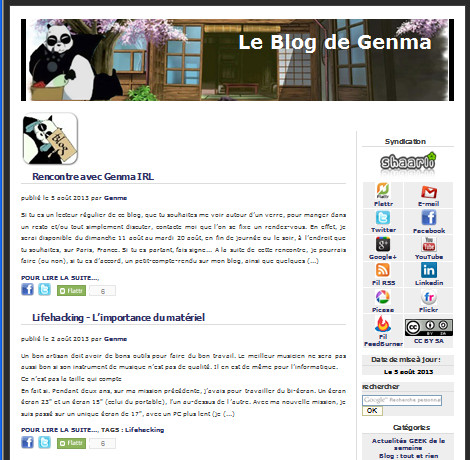
\includegraphics[width=5cm,height=5cm]{./blog.jpg} 

\end{columns}
\end{frame}

%----------------------------------------------------------------------------------------
\begin{frame}
\begin{center}
\Huge{Privacy Café}
\\~\\

\includegraphics[width=3cm,height=3cm]{./CryptopartyGenericLogo.jpg} 
\end{center}
\end{frame}

%------------------------------------------------
\begin{frame}
\frametitle{What is privacy cafe?}
\begin{block}{Privacy café, cryptoparty ...}
\justifying{
First there was the cryptoparty term (contraction of crypto - encryption and party). But now we use the term privacy café, which is less connoted version of this term. Connoted in the sense that cryptoparty is closely linked to the world of hackerspaces, underground ...
}
\end{block}
\end{frame}

%------------------------------------------------
\begin{frame}
\frametitle{When does it start?}

\begin{block}{Once upon a time...}
\begin{itemize}
\justifying{ 
\item The cryptoparty longstanding. But it was in October 2013  was launched the first privacy Café,  in Paris, France.
\item Since then, at least one event held every month.
}
\end{itemize}
\end{block}
\end{frame}

%------------------------------------------------
\begin{frame}
\frametitle{Who is affected?}

\begin{block}{What is the target / audience for Privacy Café?}
The target audience of privacy cafés is diverse and varied :
\begin{itemize}
\justifying{
\item Journalists and other risky jobs;
\item Less School (High school students, students);
\item Geeks, techies and other...;
\item But mostely everybody.
}
\end{itemize}
\justifying{
In general, it can be anyone aware / concerned with issues of privacy, security of his communications ...
}
\end{block}
\end{frame}

%----------------------------------------------------------------------------------------
\begin{frame}
\begin{center}
\Huge{How's it going?}
\\~\\

\includegraphics[width=3cm,height=3cm]{./CryptopartyGenericLogo.jpg} 
\end{center}
\end{frame}

%------------------------------------------------
\begin{frame}
\frametitle{Privacy cafés concept}

\begin{block}{Where, who, what?}
\justifying{
Just a place to meet, animators willing to share their knowledge and a public eager to learn more, who wants to learn.
}
\end{block}
\end{frame}

%------------------------------------------------
\begin{frame}
\frametitle{Workshops, talks, debates}

\begin{block}{Progress type of a privacy café}
\justifying{
At first, we did a quick overview of topics that can be discussed. Then, groups are formed and then held:
\begin{itemize}
\item  a (ligthning) talk;
\item workshop (each installs and handles on his own machine);
\item  debate, Question/Response meeting
\end{itemize}
The ideal duration is one hour and a half. With two sessions is filled afternoon.
}
\end{block}
\end{frame}

%------------------------------------------------
\begin{frame}
\frametitle{Software 1/2}

\begin{block}{Free Software}
\justifying{
The tools are all compatible with Linux, Windows and Mac and / or they have alternatives. We also talks about the problems on smatphone.
\begin{itemize}
\item Whenever possible, it is free software which is preferred. Each comes with their computer and whatever the operating system(Linux GNU \ /, MacOSX, Windows, Android), most software suitable are installed.
\item But we explain that Apple, Windows and Android pose the problems of not being free systems. So we can not trust their.
\end{itemize}
}
\end{block}
\end{frame}

%------------------------------------------------
\begin{frame}
\frametitle{Software 2/2}

\begin{block}{Free Software}
\justifying{
\begin{itemize}
\item Windows and Apple are more than strongly discouraged in the context of trust and crypto.
\item Make crypto on it, it's a bit like having an armored door to your house, but with cardboard walls.
\end{itemize}
}
\end{block}
So we are considering to so some sessions of Install party to put a less a double boot ...
\end{frame}

%------------------------------------------------
\begin{frame}
\frametitle{The proposed workshops}

\begin{itemize}
\justifying{
\item How to Encrypt emails using GPG;
\item Write and surf anonymously using TOR (Tails, TorBrowser Bundle);
\item How to protect the browser and understand the security certificates (SSL);
\item Understand and use a VPN;
\item Protect communications and surfing. Laptop and smartphone mobile (wifi and tools);
\item Protect information with TrueCrypt;
\item Passwords and multi-factor identification;
\item Identify and know how to manage or delete the metadata
}
\end{itemize}
Anything that has to do with privacy ...
\end{frame}

%----------------------------------------------------------------------------------------
\begin{frame}
\begin{center}
\Huge{Privacy cafés organisation}
\\~\\

\includegraphics[width=3cm,height=3cm]{./CryptopartyGenericLogo.jpg} 
\end{center}
\end{frame}

%------------------------------------------------
\begin{frame}
\frametitle{Privacy Café are cryptoparty}

\begin{block}{The concept is not new ...}
\justifying{
As mentioned in the introduction, cryptoparties existed for some years. Privacy Café are "just" a modern version.
}
\end{block}
\end{frame}

%------------------------------------------------
\begin{frame}
\frametitle{Organize}

\begin{block}{Who can organize a privacy café?}
\begin{itemize}
\justifying{
\item Anyone who has the basic knowledge and want to share can engage in the implementation of its own privacy coffee.
}
\end{itemize}
\end{block}

\begin{block}{What are the likely places to host a coffee privacy?}
\begin{itemize}
\justifying{
\item   
Privacy Café is aimed at a diverse audience, from mainstream to more advanced users, the site can be libraries, computer fairs ...
}
\end{itemize}
\end{block}
\end{frame}

%------------------------------------------------
\begin{frame}
\frametitle{Logistics}

\begin{block}{What are the logistics of a privacy café?} 
\justifying{The following items were identified: }
\begin{itemize}
\justifying{
\item know the capacity of the place, have one or several reference contacts;
\item provide online registration (to assess the number of participants) on a tool anonymous;
\item provide access to the Internet via a wired network (Ethernet cable + switch) and / or WiFi;
\item provide chairs, tables, extension cords in sufficient quantity;
\item a video projector ...
}
\end{itemize}
\end{block}
\end{frame}

%------------------------------------------------
\begin{frame}
\frametitle{Communication}

\begin{block}{Which slogans can be used to promote privacy coffee?}
\begin{itemize}
\justifying{
\item Learn how to protect your online communications!
\item Encryption and anonymity : regain control of your privacy.
\item Surf and chat with nice cypherpunks.
}
\end{itemize}
\end{block}

\begin{block}{Or}
\begin{itemize}
\justifying{
\item Because preserving privacy is a right,
\item Because you might want not to be spied
\item Because we ALL have something to hide,
\item Because the tools exist and are not so complicated ...
\item Learn how to protect yourself online!
}
\end{itemize}
\end{block}
\end{frame}

%------------------------------------------------
\begin{frame}
\frametitle{Advice}

\begin{block}{Some tips for the conduct of the privacy café?}
\begin{itemize}
\justifying{
\item Adapt to the participants level (from beginner to advanced user).
\item Consider the needs and expectations of the public.
\item In early trading, a small survey / round sets expectations and workshops that will be put in place.
\item The recommended duration for workshops is 1:30.
\begin{itemize}
\justifying{
\item Two successive workshops seem enough to start.
}
\end{itemize}
\item Attention to pictures / recordings etc..
}
\end{itemize}
\end{block}

\begin{block}{Do not forget the primary objective}
\begin{itemize}
\justifying{
\item We're not a IT support.
}
\end{itemize}
\end{block}
\end{frame}

%------------------------------------------------
\begin{frame}
\frametitle{Why don't you launch a privacy café?}
\begin{block}{How help, contribute...}
\begin{itemize}
\justifying{
\item Start in your city, your association, LUG ....
\item Communicate, talk about it around you.
\item Post an article (blogger, reporter ...)
}
\end{itemize}
\end{block}

\begin{block}{The cryptoparty are multiplying}
\justifying{
Toronto, Fribourg, Tokyo, Belgium, Holland...
Also in France in Paris, Toulouse, Nantes, Brest...
}
\end{block}

\begin{block}{May I help you?}
\justifying{
I'm french and I publish all my talks, tutorials, blog post under CC licence.
Help me or enjoy yourself to translate in English! ;-)
}
\end{block}
\end{frame}

%----------------------------------------------------------------------------------------
\begin{frame}
\begin{center}
\Huge{Positives points\\ of privacy cafés}
\\~\\

\includegraphics[width=3cm,height=3cm]{./CryptopartyGenericLogo.jpg} 
\end{center}
\end{frame}


%------------------------------------------------
\begin{frame}
\frametitle{Knowledge sharing}

\begin{block}{Positives points}
\begin{itemize}
\justifying{
\item Reappropriation of computers by the general public
\item Awareness to the issues of privacy, encryption ...
\item Learning how the Internet works ...
\item Raising the level of general knowledge 
\begin{itemize}
\justifying{
\item People come back and ask more specific more technical question ...
}
\end{itemize}
}
\end{itemize}
\end{block}
\end{frame}
  
%----------------------------------------------------------------------------------------
\begin{frame}
\begin{center}
\Huge{Issues of privacy cafés}
\\~\\

\includegraphics[width=3cm,height=3cm]{./CryptopartyGenericLogo.jpg} 
\end{center}
\end{frame}

%------------------------------------------------
\begin{frame}
\frametitle{Some issues...}

\begin{block}{Can you advise encryption on proprietary software?}
\justifying{
You must present all the tools with all their limitations. And consider that the opposite person is smart enough to choose.}
\end{block}

\begin{block}{The software ergonomics}
\justifying{
Projects like Tor, Tails ... do sessions on improving the design of the user experience.
The app must adapt to the user and not vice versa.
}
\end{block}
\end{frame}

%------------------------------------------------
\begin{frame}
\frametitle{Some issues...}
\begin{block}{Creating a false sense of security}
\justifying{
A few clicks can afford to send encrypted mails (Enigmail). But we forget the problems associated with metadata, which are the really important data ...}
\end{block}
\begin{block}{Threat model}
\justifying{
Everyone has a different threat model and the cursor / level of security required will not be the same ...
}
\end{block}
And other issues that can be addressed in the heckle question that will follow ...
\end{frame}

%----------------------------------------------------------------------------------------
\begin{frame}
\begin{center}
\Huge{Conclusion}
\\~\\

\includegraphics[width=3cm,height=3cm]{./CryptopartyGenericLogo.jpg} 
\end{center}
\end{frame}
\end{document}

\end{document}